\chapter{Introduction} \label{cha:intro}
This chapter first introduces a general overview of the field of Visualization with its benefits, drawbacks, and dangers in order to provide context for the rest of this thesis.  Second, a commonly used version of the visualization pipeline is introduced including some of its attributes and modifications.  The third section presents a short overview of interaction design and its requirements regarding the design of systems where the human-in-the-loop approach is essential.  The last section provides an overview of visualization systems which include a classification system that is based on the target audience and usage for which a system is designed.

This chapter is not exhaustive by any means and the inclined reader searching for more detailed information is referred to a number of books for a broader overview of the field.  A general overview of the design of visualization applications is provided by Munzner~\cite{munzner2014visualization}.  Specificially for medical applications, Preim and Botha~\cite{preim2013visual} provide a detailed outline of the use of visual analysis in medicine.

\section{Visualization} \label{cha:intro:vis}
Throughout the years, there have been many attempts at finding a universally accepted definition of the scientific, design, or engineering discipline \emph{Visualization}.  Card~\etal~suggested that Visualization is ``the use of computer-supported, interactive, visual representations of data to amplify cognition''~\cite{card1999readings}.  Other definitions, however, place their focus on the interplay between generated images and the process of subjective visualization in each person~\cite{van2006views}, or generalize the concept of visualization to non-visual phenomena as well~\cite{ronnberg2016interactive}.  While these definitions vary widely, their commonality is the focus on a human observer and the fact that a visualization is created for and by a human, which inherently requires understanding of human physiology and decision making.  Furthermore, the field of visualization was started as, and continues to be, a reaction to the data explosion occurring in other fields~\cite{lorensen2004death}, as a means to make sense of the vast quantities of data that these fields regularly generate and that exceed the human capacity for understanding.

The field of visualization is often separated into at least three categories;  \emph{Scientific Visualization}, \emph{Information Visualization}, and \emph{Visual Analytics}.  Scientific Visualization is characterized by the use of data sources with an inherent physical and spatial component.  Data traditionally attributed to Scientific Visualization comes in the form of, for example, simulations or datasets in which the spatial relationship is trivially given.  Information Visualization usually deals with abstract data that does not need to possess an innate spatial component.  Techniques from this part are typically high-dimensional and multi-variate.  Visual Analytics places heavier focus on the analytical reasoning and the interaction modes in order to produce insight into the data rather than the source of the data itself~\cite{wong2004guest}.

\noindent According to Tory~\etal~\cite{tory2002model}, these definitions require the use of words such as ``usually'', ``typically'', or ``traditionally'' which hints at a problem with this type of classification.  For once, it is not always possible to delineate differences between the categories even in the most trivial applications of visualization~\cite{rhyne2003information, weiskopf2006scivis}.  More complicated applications almost always use research from two or all three categories, increasing the difficulty of a clean classification.  Additionally, from an application domain's point of view, the distinction between different fields might not even be noticable or relevant.  In their work, Tory~\etal~provide a more nuanced \emph{model-based taxonomy} that is focusses on the characteristics of the model of the data rather than the data itself.  Instead of using a taxonomy that is based on the description of the data, they propose a taxonomy that is based on the way the data is used in the visualization system and differentiates between \emph{continuous} and \emph{discrete} data, regardless of whether the data itself is abstract or spatial.  In this thesis, there is no distinction between the visualization categories as they are providing different tools to solve the same class of problems, that is, displaying data to a human in order to facilitate insight, and ``at this level there is much more they share than what separates them''~\cite{van2006views}.

\subsection{Benefits of Visualization} \label{cha:intro:vis:benefits}
As mentioned in the previous chapter, humans are exceptionally well adapted to interpret information contained in images.  This is exemplified by the popular quote that ``a picture is worth a thousand words'', meaning that, for humans, the bandwidth to ingest information visually is much higher than through other representations.  However, the computational complexity of problem classes might differ between the human visual system and computational operations.  This leads to the realization of two classes of problems.  On the one hand, there are problems that can be solved more efficiently by computers, such as searching large databases and algorithms that typically operate on a map-and-reduce scheme.  On the other hand, there are problems solved better by humans, such as pattern recognition, hypothesis forming, and others.  An example of this is detecting proximity among a group of objects, which for the human perception method is of constant complexity ($\mathcal{O}\left( 1 \right)$), and for an algorithm at best linear ($\mathcal{O}\left( n \right)$).  Visualization, being placed on the boundary between these two problem classes, can utilize the respective strengths of both computers and humans through a close integration in order to solve a larger problem set efficiently.

\subsection{Limitations and Dangers of Visualization} \label{cha:intro:vis:limitations}
One of the important limiting factors influencing each visualization is its subjectiveness.  According to van Wijk, the benefit of using a visualization depends on ``the specification [...], the perceptual skills of the observer, and the a priori knowledge of the observer''~\cite{van2005value}.  This realization is yet another reason why close collaboration between the visualization designer and the domain expert is of fundamental importance, as the design process has to take the experts a priori knowledge into account.  Lorensen elaborated on the potential problems for the visualization community that could arise if this collaboration does not occur and summarized it as ``[Visualization] has lost its customers''~\cite{lorensen2004death}.  The fact that visualization is still alive over a decade later indicates that it indeed was possible for visualization to maintain this close collaboration.  Another direct consequence of the subjectiveness is that the reproducibility of a visualization is limited to comparable consumers.  A visualization system that is designed for experts in a specific field loses much of its applicability when applied to the same data models from a different field.

Another aspect of the a priori knowledge that is often overlooked is a dependence on cultural background.  Whereas knowledge-based prior information can be assessed empirically, it is much harder to assess cultural bisases.  Some of these cultural differences can be benign, such as the Western tendency to associate movement across a red-green color scale with an increasing value, whereas East Asian cultures would associcate this with a decreasing value, due to the flipped association between the red and green colors.  Other differences can be seen in \fref{fig:intro:vis:lego}, which displays characters from eight cartoon series built from Lego blocks and can be seen as a form of visualization.  Viewed in a culture that is unfamiliar with these cartoon series, however, it becomes easy to see that this visualization will be unable to produce any meaningful results to that group of users.

\begin{figure}
  \centering
  \fbox{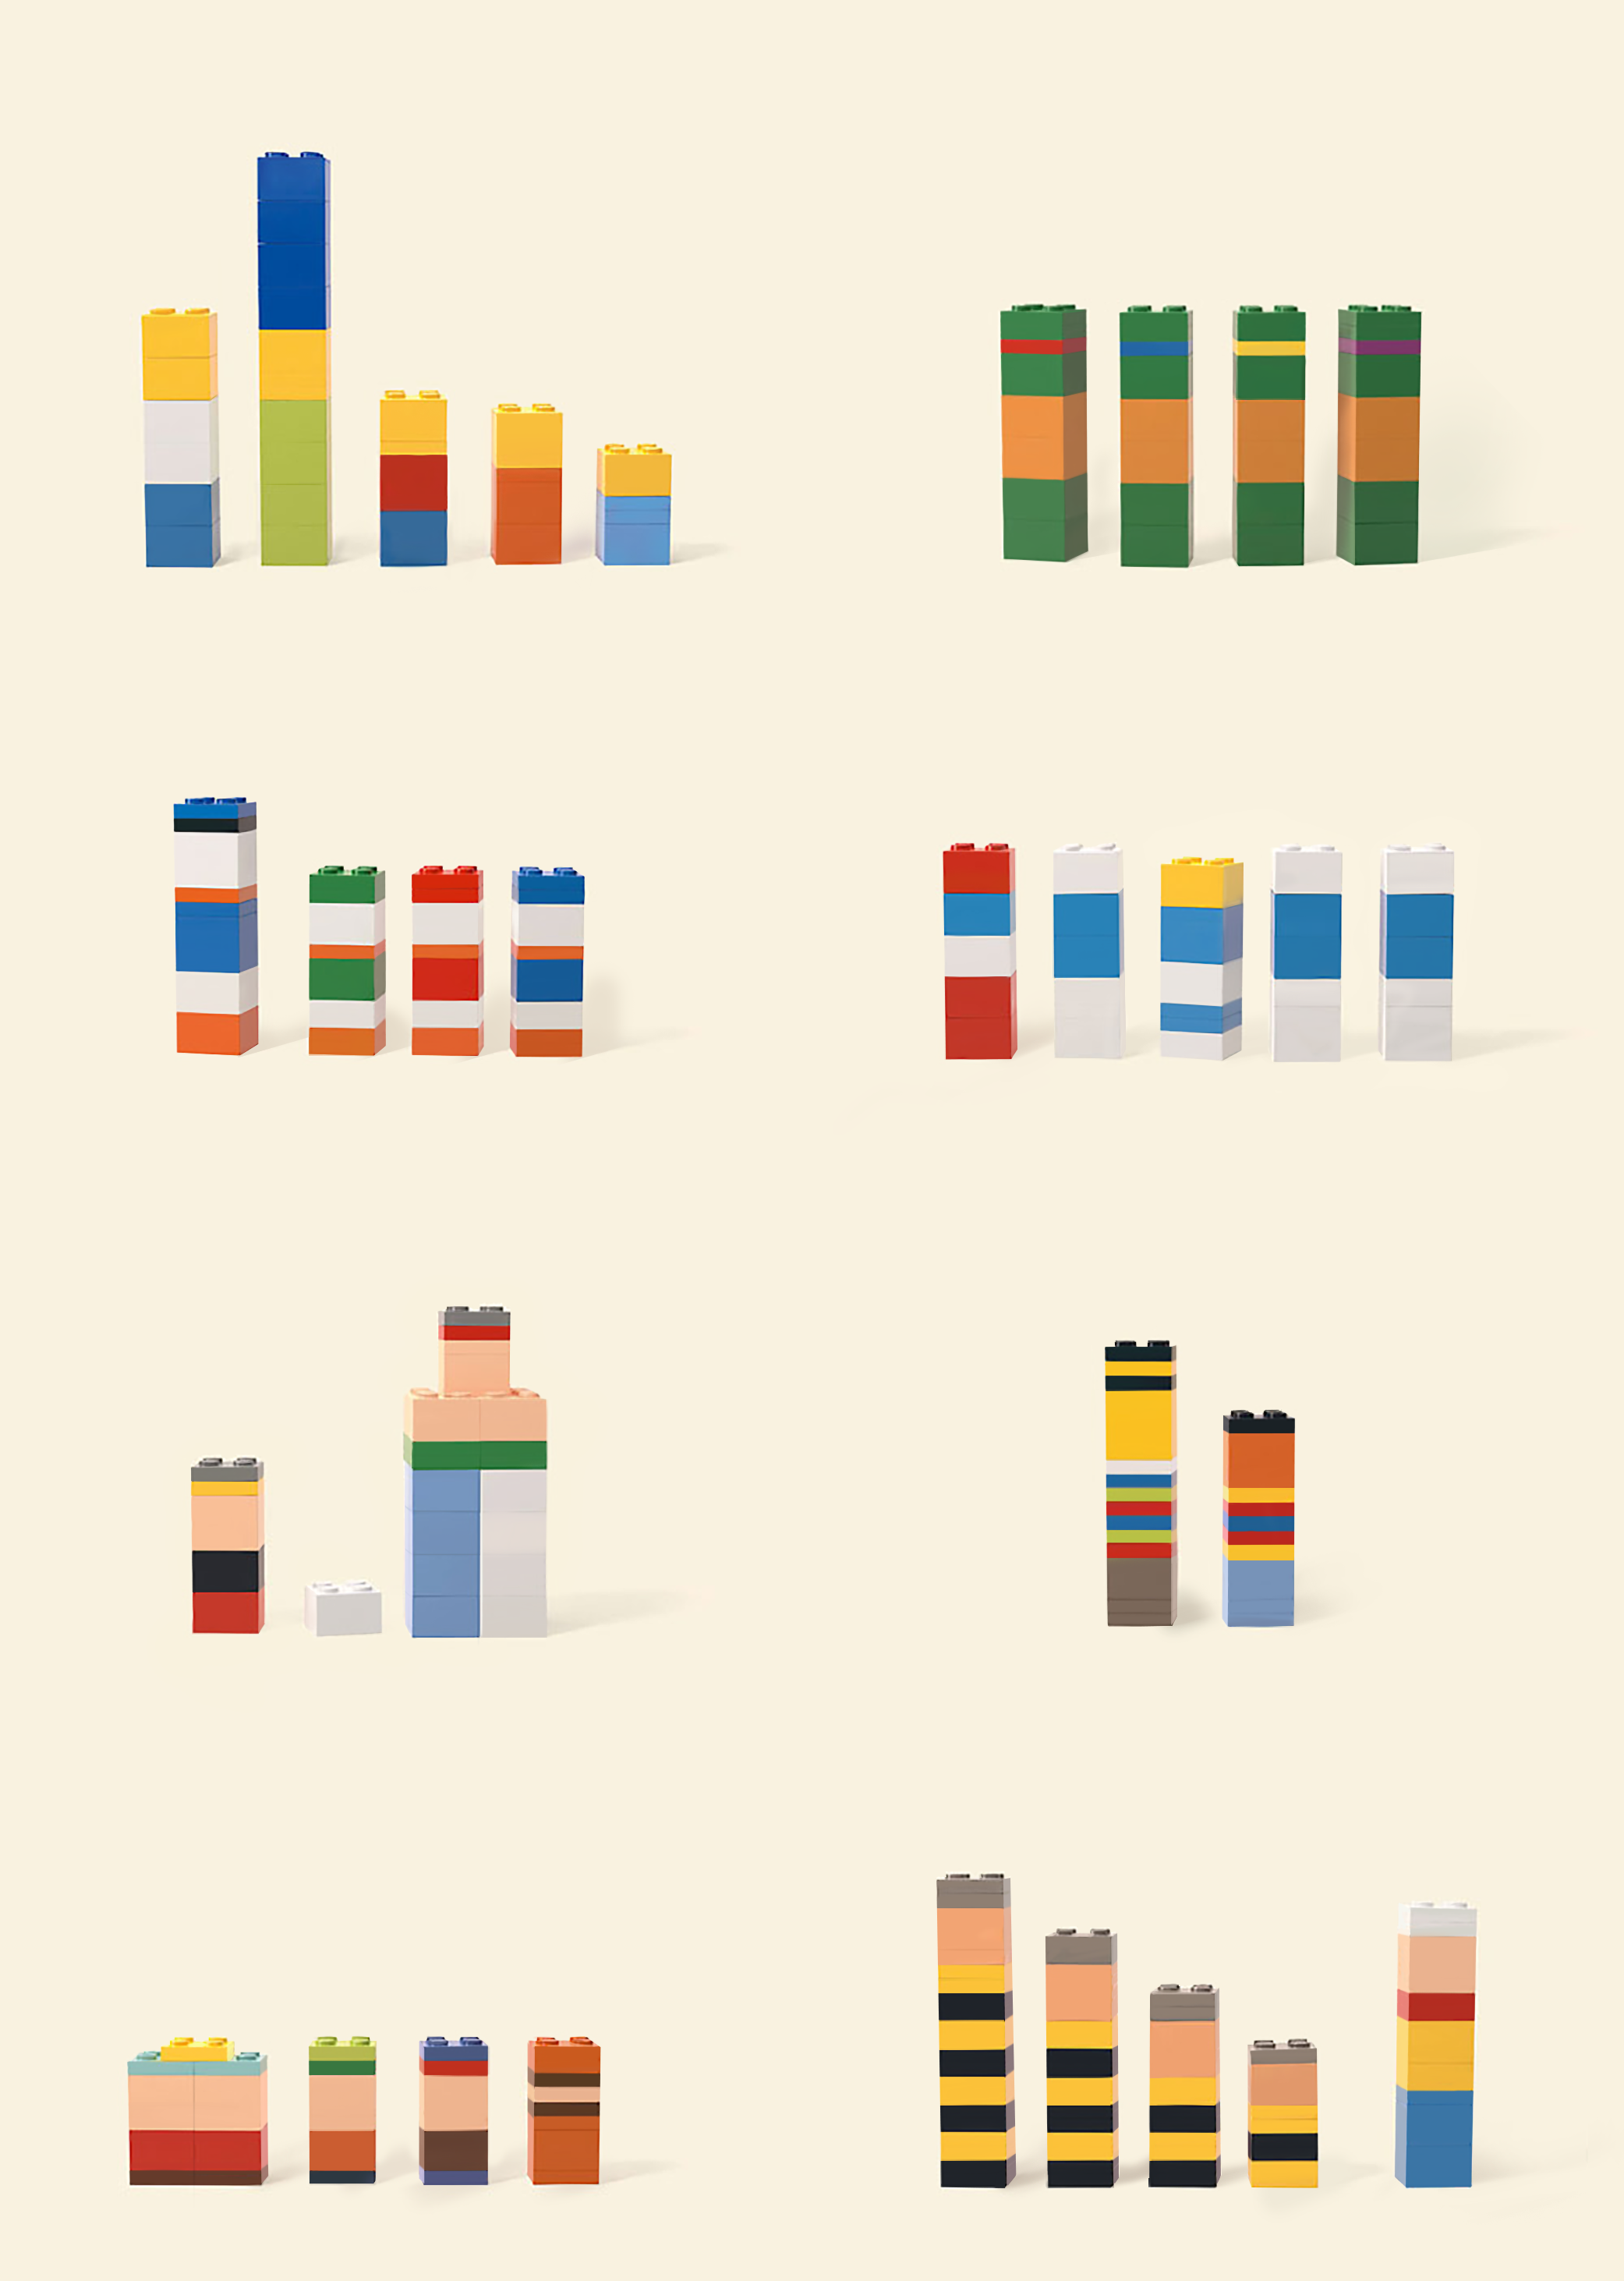
\includegraphics[width=0.5\textwidth]{figures/intro/lego.png}}
  \caption{A collection of advertisement images representing cartoon characters. With the required cultural background, deciphering these visualizations is impossible. Image copyright by Lego.}
  \label{fig:intro:vis:lego}
\end{figure}

% \subsection{Dangers} \label{cha:intro:vis:dangers}
Beside the immense benefits that visualization can provide for supporting data interpretation and hypothesis testing, the misuse of visualization can have a detrimental effect and pose a danger to the acquisition of insight.  One obvious aspect outside the scope of this thesis is the use of visualization to deliberately mislead the audience.  Even without a deliberate attempt, there are many pitfalls that need to be considered when designing a visualization.  Verifying truths, rather than inspiring hypotheses can easily lead to confirmation biases that might lead experts to draw faulty conclusions, exemplified in the quote from van Wijk saying that ``visualization should not be used to verify the final truth, but rather to inspire to new hypotheses, to be checked afterwards''.  Naturally, this danger is most prevalent in the initial exploration stages of a visualization and can be mitigated when a visualization system is matured and applied to many of the same types of datasets; nevertheless, it is an important aspect to consider during the design process.  The remaining dangers fall into one of two categories, \emph{showing incorrect information} and \emph{showing information incorrectly}.  The first category can occur if visualization designers apply wrong assumptions about the data by, for example, applying smoothing to inherently discrete data sets, not handling outliers correctly in a filtering operation, or not considering missing data in real world datasets.  For the domain expert it then becomes difficult to differentiate missing data from outliers, thus eroding their trust in the visualization system.  In the second category, color maps play a huge role.  Ill-suited color maps trivially enable the possibility to highlight or hide structures in the data without informing the expert about the process.  One example is the continued use of the rainbow color map in science publications even though it has been shown to be inferior to other color maps~\cite{borland2007rainbow}.



\section{The Visualization Pipeline} \label{cha:intro:vp}
\begin{figure}
  \centering
  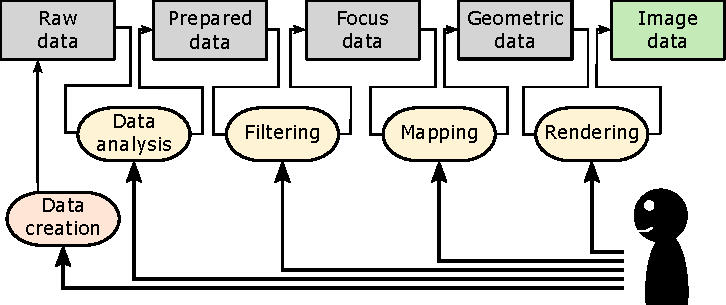
\includegraphics[width=\textwidth]{figures/intro/pipeline.pdf}
  \caption{One version of the visualization pipeline as described by Dos Santos and Brodlie~\cite{dos2004gaining}.  The acquired data is repeatedly transformed until an image is generated that can be used by the user to gain insight.  The user's ability to control each part of the visualization pipeline is at the heart of the human-in-the-loop methodology.}
  \label{fig:intro:vp}
\end{figure}

\fref{fig:intro:vp} shows a schematic overview of the visualization pipeline.  All fundamental visualization research aims to improve or impacts one or more stages in the visualization pipeline and all applied visualization research and systems utilize the concept of this pipeline.  The pipeline used was first described by Haber and McNabb in 1990~\cite{haber1990visualization} and later extended by Dos Santos and Brodlie in 2004~\cite{dos2004gaining}.  It consists of four transformations that are successively applied to the incoming data.  For a complete description of the visualization pipeline and its variations, we refer to the two original works or by a survey about the development of the visualization pipeline by Moreland~\cite{moreland2013survey}.

The input to the pipeline is the \emph{Raw data} that is acquired from measurements or simulations.  This data can be structure or unstructured, static, or time-varying.  It is processed by the initial \emph{Data analysis}, which consists of resampling, interpolation, or removal of outliers.  In the \emph{Filtering} step, the data is reduced with respect to the requirements of the specific task that is to be solved, for example thresholding, level-of-detail selection, or segmentation.  This \emph{Focus data} is then converted in the \emph{Mapping} stage into what Haber and McNabb referred to as \emph{Abstract Visualization Objects}; an abstract object that contains visualization-related attributes, such as color, geometry, or texture, that depend on, but do not necessarily correspond to, the input data.  The final step, \emph{Rendering} uses these abstract representations and generates a final image.%It is only in this last step, where the details of a rendering framework and algorithms, such as OpenGL, are used extensively~\cite{segal2016opengl}.

One important aspect for the design of visualization applications that was not fully accounted for in the original visualization pipeline is the feedback from the user into the various transformation stages.  While it has been possible to change the parameters of the \emph{Rendering} or \emph{Mapping} stages by, for example, changing the camera position, or changing the color attributes of the Abstract Visualization Objects of Geometric Data, for a long time, the focus of interactivity for the other steps of the pipeline has been introduced later.  One of the last feedback loops, Computational Steering, described by Mulder~\etal~\cite{mulder1999survey}, enables the visualization user to directly influence the gathering of the \emph{Raw Data} and inspect the results with minimal delay.  Closing this loop leads to the biggest gain in insight as the user can, in the example of simulations, directly understand the influence of parameter changes and can thus gain a deeper understanding of the origin of the data.

\begin{figure}
  \centering
  \fbox{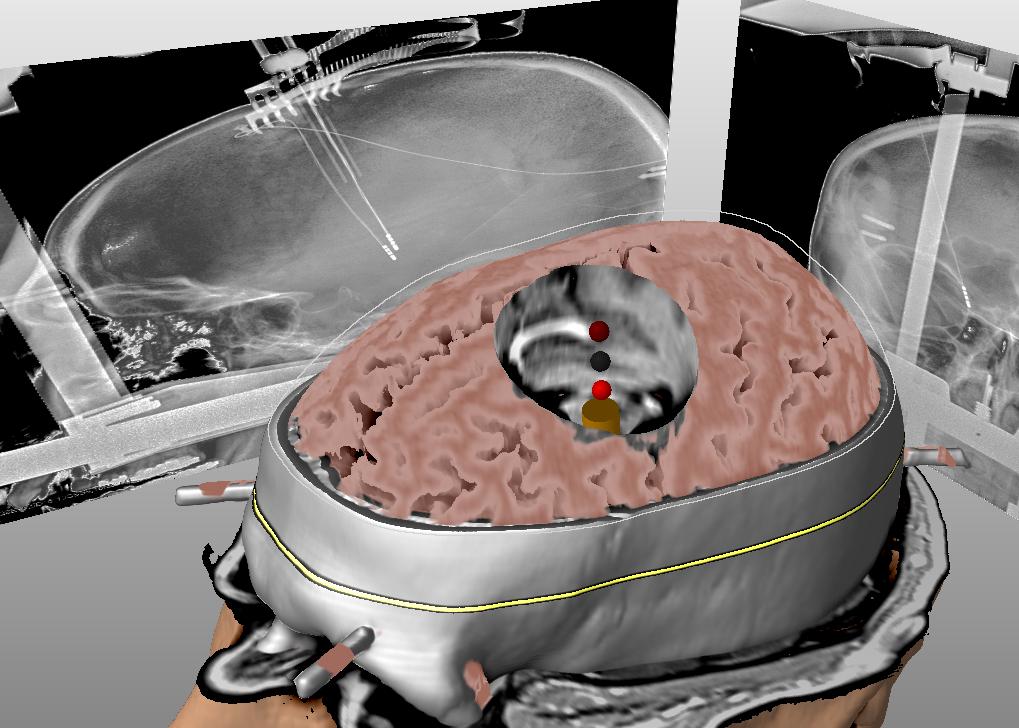
\includegraphics[width=0.65\textwidth]{figures/intro/magicmirror.png}}
  \caption{One example of a multiview visualization technique, a \emph{Magic Mirror}, where X-ray scans of a patients are shown projected to the sides of a combined volumetric rendering.}
  \label{fig:intro:mm}
\end{figure}

An important aspect of the design of visualization systems that is hidden from the pipeline depicted in the figure is the possibility of pipeline branching.  Multiview visualization systems provide multiple simultaneous views on complementary aspects of the data.  One example of these techniques is a magic mirror~\cite{konig1999multiple} as shown in \fref{fig:intro:mm} that presents different aspects of the underlying data projected to the sides of a surrounding cube, thus providing the expert with additional simultaneous information about the data.  In a multiview system, separate branches of the pipeline handle these views that are ultimately merged in the \emph{Rendering} step.  There exists a large amount of research on techniques dealing with multiview systems, an example of which is brushing or linking~\cite{tory2003mental}.



\subsection{Data Acquisition} \label{cha:intro:vp:da}
Regardless of its exact composition, the visualization pipeline starts with data that is either collected and measured from the real world or generated by simulations.  While in the abstract, the specific form and shape of the data does not influence the visualization pipeline, concrete systems require knowledge about the origin and characteristics of specific data sources.  This section elaborates on some of the attributes that are important for the contributions included in this thesis.

\subsubsection{Data structures} \label{cha:intro:vp:da:datastructures}
There is a variety of methods to structure the acquired data.  This section introduces a subset of data layouts with a focus on representations that are used in this thesis.  This is by no means a complete reference as each specific problem domain can demand its own optimal data representation.

\paragraph{Point Cloud. }  Sparse point cloud data is the least structured of these data types and consists of, potentially multi-dimensional, measurements in a \nD{2} or \nD{3} space that in general do not possess any information about their connectivity.  Lidar scanners are a prime example of a modality that generates unstructured point cloud.  Point clouds, due to their unstructured storage, are difficult to handle and thus pose unique visualization challenges, such as handling transparency, occlusion, and the need for efficient rendering techniques.

\paragraph{Cartesian. }  Multidimensional Cartesian grids are the most widely used form of structured data, with \nD{3} volumetric grids being the most applicable to this thesis.  The uniform structured grid makes it possible to efficiently handle a large amount of data.  A large number of techniques to render this data type exist, for example isosurface rendering or \emph{direct volume rendering}.  The ubiquitious nature of Cartesian volumetric grids also provides a major drawback.  Since it is the de facto standard data format in Scientific Visualization, it is often used in domains that are not space-filling or where an adaptive resolution would be more appropriate, thus resulting in suboptimal storage and access methods where an adaptive grid or a different underlying geometry would be better suited.

\paragraph{Spherical. }  One non-Cartesian grid structure that is used in this thesis is a grid based on spherical coordinates.  Simulations of the inner solar system produce higher resolution closer to the origin and automatically possess a spherical symmetry which can be utilized to optimize storage capacity.  In these cases, a spherical data set is a \nD{3} volume, where each of the three spherical coordinate axis, $r$, $\phi$, and $\theta$ is mapped to a respective Cartesian axis.  When applying direct volume rendering techniques to these datasets, interesting characteristics, such as automatic adaptive sampling or spherical linear interpolation schemes, can be observed~\cite{balabanian2007sonar}.

\subsubsection{Dimensionality} \label{cha:intro:vp:da:dimensionality}
Unfortunately, the word \emph{dimensionality} is overloaded many times in Visualization.  For this section, dimensionality refers to the number of values stored at each location in the dataset, rather than the number of dimensions of the dataset itself.  For the purposes of this thesis a taxonomy, for example as provided by Shneiderman~\cite{shneiderman1996eyes}, is used that describes data as \emph{scalar}, \emph{vector}, \emph{tensor}, or \emph{multi-dimensional}.  The difference between a \nD{3} dataset and a vector dataset is that a vector has additional inherent information that can, and should, be used to restrict the creation of Abstract Visualization Objects.

Each of above categories can also be \emph{time-varying}.  While there have been many techniques that efficiently deal with time-varying datasets, for example time-space partitioning trees~\cite{shen1999fast}, efficient handling of these datasets has not been the focus of this thesis.  As such, this work handles the temporal dimension analogous to the already existing spatial dimensions and, thus, a time-varying dataset as an ordered series of single timestep datasets.

\subsubsection{Data Sources} \label{cha:intro:vp:da:sources}
There are countless potential sources of datasets and a conclusive enumeration would exceed the scope of any single work.  Instead, this section is presenting a brief overview of the different data modalities and their data acquisition techniques that are being utilized in the contributions section.

\paragraph{X-ray. } X-ray radiation was discovered by Wilhelm R\"ontgen in 1896~\cite{rontgen1896xray} and was quickly developed into an imaging technique.  A \emph{source} emits radiation that passes through the object of study.  The constituent materials' absorption coefficients determine the amount of radiation that is absorbed when passing through the object.  A photographic plate on the other side of the object captures the remaining intensity and thus reconstructs a representation of the object's radiotransparency.  The limitation with this technique is its restriction to a single \nD{2} projected image of the object in question and can thus not be easily used for a \nD{3} reconstruction.

\paragraph{Computed Tomography. }  A Computed Tomography (CT) scanner works similar to an X-ray detector, in which the source and an electronic detector are rotating around the imaged object.  Throughout this motion, many images are taken by the scanner, which are then reconstructed into a single \nD{3} representation of the object in question.  The Nobel Prize for Physiology or Medicine was awarded to Hounsfield and Cormack in 1979 for their development of this machine~\cite{hounsfield1980computed}.  The spatial and temporal resolution of the scanner and technique has since been improved by multiple orders of magnitude, enabling current machines to perform full-body scans of patients in only a few seconds, or provide the ability to scan a smaller area of interest multiple times per second, thus extending the available information from the structural aspect into the functional domain.  In medical applications the X-ray attenuation is measured in \emph{Hounsfield Units} that measure the attenuation factor of materials and thus provides a standardized scale.  As the X-ray attenuation between different soft tissues is not very high, it is most widely used to study the skeletal structure in humans.

\paragraph{Magnetic Resonance Imaging. }  Magnetic Resonance Imaging (MRI) scanners operate by rapidly manipulating magnetic fields to force an alignment of the spins of hydrogen atoms and measuring the time it takes an atom to fall back to the ground state.  The radio frequency emitted by this process is detected by the scanner and used to reconstruct a \nD{3} volumetric representation of the object of study.  Since the signal is based off the availablility of hydrogen atoms, MRI scans exhibit the highest resolution in areas with a high water content, such as soft tissue in human patients, whereas the skeletal structure is not well captured~\cite{damadian1971tumor}.  Comparing these attributes to a CT scanner shows that combining CT/MRI scanners provides a high resolution scanner result for a large part of the human body, thus the combination of these two modalities is often used in practice.

\paragraph{Lidar. }  A Lidar scanner is another active scanning device that uses light to a similar effect as radar uses radio waves.  It operates by emitting coherent light and measuring the time until the reflected light returns to the detector, thus making it possible to create a \nD{3} line-of-sight representation of the area surrounding the scanner.  These measurements can be used to create a high-resolution \nD{3} model of, for example, humans or building structures.  Combining a Lidar scanner with other scanning modalities, it becomes possible to not only detect the presence or absense of an obstacle, but also measure other physical attributes, for example surface temperature by measuring radiation emitted by an object or radial velocity through doppler shift.  One important use case for Lidar scanners are autonomous vehicles that can use this information to generate an accurate, real-time \nD{3} local environment that can be used for navigation.

\paragraph{Simulations. }  The previous modalities generate data by measuring physical quantities and thus create a virtual representation of a physical phenomenon which can then be visualized.  Simulations, on the other hand, utilize a minimal set of physical preconditions and try to recreate the physical world and thus enable insight into areas that would either be infeasible or impossible to investigate directly.  This enables the recreation of phenomen\ae that all possible scales, but are especially useful in which direct measurements are challenging.  An important distinction between the measured modalities and simulations arises in the form of noise that is introduce into the data.  Whereas simulations have the potential for a very low signal-to-noise ratio, any measured modality will always have some form, or multiple forms, of noise attached to the signal that have to be considered in the visual representation.



\subsection{Direct Volume Rendering} \label{cha:intro:vp:dvr}

\begin{wrapfigure}{o}{0.4\textwidth}
\centering
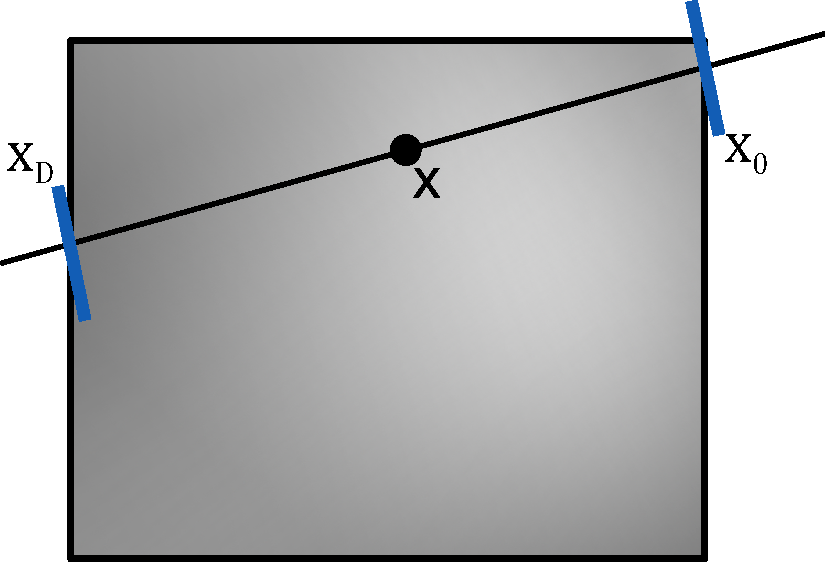
\includegraphics[width=0.39\textwidth]{figures/intro/rendering_integral.pdf}
\caption{Illustration of the rendering integral for a ray with entry point $\vec{x_0}$, exit point $\vec{x_D}$ and an exemplary sampling point $\vec{x}$}
\label{fig:intro:dvr}
\end{wrapfigure}

Most of the work presented in this thesis deals with \nD{3} volumetric data sets for which \emph{direct volume rendering}~(DVR) is a very well-suited and well-established rendering algorithm. It was derived from simplifying general ray tracing algorithms and thus enabling the possibility to be computed at interactive frame rates.  Traditionally, DVR uses a simple emission/absorption model that assumes that the volume is composed of small particles that each have the ability to emit and absorb light, and thus is considered a participating medium~\cite{levoy1988display, drebin1988volume, sabella1988rendering}.  The mathematical formulation of the incoming radiance $I$ was first described by Max~\cite{max1995optical, max2010local}.  Using the definitions in \fref{fig:intro:dvr}, this results in:
\begin{equation}
I(\vec{x_c}) = \underbrace{I_0 \left( \vec{x_0} \right) T\left( \vec{x_0}, \vec{x_D} \right)}_{\textrm{Background}} + \int_\vec{x_0}^\vec{x_D} \underbrace{\sigma_\alpha(\vec{x}) I_c(\vec{x})}_{\textrm{Contribution}}  \underbrace{T(\vec{x}, \vec{x_D})}_{\textrm{Attenuation}} \textrm{d} \vec{x},
\label{eqn:intro:dvr}
\end{equation}
\noindent where $I_0$ determines the background illumination, $\sigma_\alpha$ determines whether a sample $\vec{x}$ is emitting or absorbing light and $I_e$ specifies the amount of light contributed at a location $\vec{x}$, attenuated by the attenation factor $T$, given by:
\begin{equation}
T(\vec{a}, \vec{b}) = \exp \left( -\int_\vec{a}^\vec{b} \tau(\vec{x}) \textrm{d} \vec{x} \right),
\label{eqn:intro:dvr2}
\end{equation}
\noindent with $\tau(\vec{x})$ being the extinction coefficient that defines the occusion of light within the volume.  Equations \ref{eqn:intro:dvr} and \ref{eqn:intro:dvr2} combined are known as the volume rendering integral.  For real-world datasets, solving the volume rendering integral analytically is not feasible and are, in practical calculations, approximated as Riemann sums with a stepsize $h$ between individual samples.  $h$ is a constant value whose value should be influenced by Nyquist's theorem~\cite{shannon1949communication}.

Many volume rendering techniques can be expressed through modification of Equations~\ref{eqn:intro:dvr} and \ref{eqn:intro:dvr2} or their finite integration step equivalent.  An example are adaptive sampling methods in which the stepsize $h$ depends on the encounted data values, thus being able to provide a higher sampling resolution in different parts of the volume~\cite{danskin1992fast}.  A specialization of this is empty space skipping, where empty parts of the volume are skipped entirely as a performance optimization method~\cite{yagel1993accelerating}.  The volume rendering integral is evaluated for each pixel in the rendering window based off the bounding geometry of the volume that is to be rendered.  By rendering the coordinates of the volume's bounding geometry and storing the results, it is possible to generate each pixel's ray and traverse it in the graphics processing unit (GPU)~\cite{kruger2003acceleration}, which has become the de facto standard in DVR.



\section{The Human-in-the-Loop Model} \label{cha:intro:hitl}
The integration of human perception, cognition, and decision making into the knowledge discovery and analysis process is a vital aspect of any visualization system.  As described by Ward \etal : ``If the goal of visualization is to accurately convey information with pictures, it is essential that perceptual abilities by considered.''~\cite{ward2010interactive}.  For human perception and cognition, examples adhering to the Gestalt theory (as mentioned in Chapter~\ref{cha:motivation}) demonstrate the vast abilities of the human visual system in recognizing clusters, independent from the number of items, based only on simple features such as color, orientation, grouping, or closure.  When designing visualization systems, it is valuable to consider the areas in which human cognition is superior to computational models and vice versa.  The paradigm of creating \emph{Human-in-the-loop} visualization system recognizes that the combination of optimal human cognition and computational models is superior to each separate mechanism~\cite{munzner2014visualization}.  In order to leverage this, the human decision maker needs to be able to influence each individual component of the visualization process.  This influences the visualization pipeline (see \fref{fig:intro:vp}) such that the \emph{Mapping} phase consists of operations that transform data into forms that are more suitable for human consumption and that the user needs to be able to change the parameters of each operation to enable an iterative knowledge gaining process.

In almost all cases the human in-the-loop is an expert in the specific application domain, the \emph{domain expert}, rather than a visualization expert.  The importance of this combination and value of visualization in these aspects has well been recognized~\cite{van2005value}.  This constellation requires the visualization system to be designed in such a way that it is easy and intuitive for the domain expert to understand and control the system and perform the desired tasks.  The design of these visualization system has undergone many studies and potential tasks have been grouped into varying groups~\cite{brehmer2014visualizing}, all of which is elaborated on in the next section.  However, it is important to acknowledge that these designs rarely succeed on the first try and require iteration, thus requiring user studies and repeated design studies, following the overall design principles of software design~\cite{larman2003iterative}.



\section{Visualization Applications} \label{cha:intro:appl}
Visualization applications are one of the large and, arguably, growing fields of research inside the visualization discipline.  As defined by descriptions at the major visualization conferences, ``An application paper normally starts with an encapsulated description of a problem domain and the questions to be resolved by visualization, then describes the application of visualization to the task, any novel techniques developed, and how the visualization solution answered the questions posed. Techniques related to a single problem are normally application papers, and evaluation is often limited because many application papers are essentially custom software for a specific problem.''

As visualization applications deal with specific needs of a user, these user groups have to be intimately involved with its design and the development.  In many cases these are single applications that combine multiple visualization techniques and, thus, amplify the contributions of each constituent component.  An example framework for this paradigm is presented by Rungta \etal\ in their ManyVis system~\cite{rungta2013manyvis}.

One widely used technique uses multiple views and linking \& brushing between the views.  The usefulness of multiview setups was shown by North and Shneiderman~\cite{north1997taxonomy}, whereas Wang \etal\ provided guidelines for their usage in visualization~\cite{wang2000guidelines}.  This includes specifying different rules, such as the \emph{Rule of Diversity}, \emph{Rule of Complementarity} and others.



\subsection{Forms of Collaborative Research} \label{cha:intro:appl:collab}
Kirby and Meyer provided an overview of different types of visualization collaborations that can be served by developing an application~\cite{kirby2013visualization}.  In particular with regard to the scientific disciplines that are involved in the project, they highlight three flavors of teams. An \emph{interdisciplinary team} consists of scientists where there is a discipline gap and thus novel problems are solved by combining techniques from multiple distinct disciplines.  \emph{Multidisciplinary} research solves challenges by tightly coupling techniques from distinct disciplines and thus enables solutions that are not solvable by each discipline alone.  Third, \emph{intradisciplinary} research is performed by collaborators from different sides of the same large discipline and fosters the internal cohesion of the scientific discipline.  Placed into the framework put forth by van Wijk, interdisciplinary and intradisciplinary teams would be placed on opposite spectrums of the \emph{knowledge gap} dimension between collaborators~\cite{van2006bridging}.

\begin{figure}
  \centering
  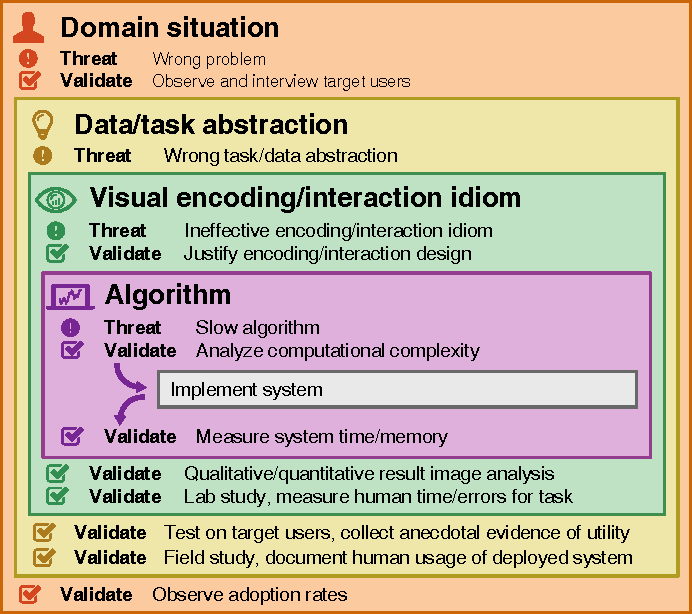
\includegraphics[width=\abfboximagewidth]{figures/intro/design_model.pdf}
  \caption{The nested model of visualization application design introduced by Munzner~\cite{munzner2009nested}\textsuperscript{1}.  Image adopted from Munzner.}
  \label{fig:intro:appl:nested}
\end{figure}


\subsection{Fundamentals of Application Design} \label{cha:intro:appl:design}
Many models describing the design of visualization applications have been published over the years.  One of the more successful models is the nested four-layer model introduced by Tamara Munzner in 2009 that describes the design of visualization applications~\cite{munzner2009nested}, to which guidelines and blocks were added in 2015~\cite{meyer15nested}.  Following this model, the design of an application consists of four sequential layers.  An error in validity of a layer impacts the downstream layers, similar to the waterfall modeling in software engineering~\cite{royce1987managing} (see \fref{fig:intro:appl:nested}).  These layers are the \emph{Domain Problem and Data Characterization}, in which the visualization designer immerses themselves in the target domain and vocabulary in order to characterize the workflow of the tasks.  In the \emph{Operation and Data Type Abstraction} layer, this knowledge is converted into a more generic computer science description of the challenges and operations that are required by the desired workflow of the domain expert.  These operations are then converted into visualization components in the \emph{Visual Encoding and Interaction Design} phase in which either novel visualization techniques are designed or previously published techniques are combined to solve the expert's particular problem.  In the last step, the \emph{Algorithm Design} all desired visual encodings are implemented to create the final system, solving potential technical challenges.

Each layer in this nested model has unique threats to its validity that influence the subsequent layers.  For example, a threat to the \emph{Domain Problem} layer would be a misclassification of the domain expert's desired workflow.  Even if the subsequent steps performed successful, the designed application will be unable to fulfill the expert's wishes and thus ultimately fail.  However, some of the validation of outer layers can only occur after the downstream layers have already been valided leading to a cascading error if the downstream layers' validation fails.

This nested layers and thread model of application design was later improved by Meyer \etal , which included more fine-grained subdivision within each layer by introducing transactional \emph{blocks} that can be identified in each layer and \emph{guidelines} that describe relationships between blocks.  Using this framework, it becomes possible to characterize the design process of an application system on an abstract level, which makes it possible to analyze and compare different application designs.


\subsection{Classification of Visualization Tasks} \label{cha:intro:appl:tasks}
One of the layers in Munzner's nested model is the ``Data/task abstraction'' layer.  Placed on the border between the abstract description of the scientific domain and the concrete details of visualization methodologies, this layer ideally lends itself to a taxonomical classification.  Like in other fields, the many proposed taxonomies across the subfields of information visualization, scientific visualization, an visual analysis show a high degree of similarity.  While concrete examples for each subfield might differ, the resulting taxonomies are similar, which points again to the fact that these subfields have more in common than what separates them.  In many of these taxonomies there exist a hierarchy of tasks, where high-level tasks such as ``confirm hypothesis'' are decomposed into groups of low-level tasks, such as ``select'' or ``filter''.  Taxonomies then combine different granularities to attempt a full description of the tasks required by a specific visualization system.  As specified by Brehmer \etal : ``Low-level classification systems often provide a sense of how a task is performed, but not why; high-level models are the converse. Our focus on multi-level descriptions of visualization tasks is intended to close this gap [...]''~\cite{brehmer2013typology}.

One of the earliest taxonomies was produced by Shneiderman in 1996~\cite{shneiderman1996eyes}, who introduced the type by task taxnomomy that focusses on the type of the data, such as number of dimensions, static vs temporal data, or organization.  It then suggests seven high-level tasks (overview, zoom, filter, details-on-demand, relate, history, and extract) that describe the kind of the operations users of a visualization want to apply to their data.  In the same paper and using the same task names, Shneiderman also coins the visualization mantra: ``Overview first, zoom and filter, then details-on-demand''.

Building on the work by Shneiderman, Schulz \etal create a design taxonomy that is a five dimensional design space that describes individual abstract visualization tasks along the dimensions of goal, means, characteristics, target, and cardinality~\cite{schulz2013design}.  The goal, providing the objective or the intended target audience is important for individual tasks as well as the visualization as a whole and is revisited in greated detail in Section~\ref{cha:intro:appl:categories}.  The means describes the method of achieving a specific goal and describes the subdivision into smaller tasks.  The characteristics describe aspects of the data that the task aims to reveal.  The target describes the kind of relations that are investigated and the cadinality describes the scope of a visualization task with regard to the data.  In addition, Schulz \etal highlight the important distinction between analyzing tasks from a visualization design perspective as visualization consisting of applying tasks to the right data (``Data + Task = Visualization'') and the evaluation standpoint asking the question which tasks are most appropriate for a particular set of data and visualization techniques (``Data + Visualization = Task'').  Similar to the design space created by Schulz \etal , a similar description was provided by Rind \etal with the proposed ``task cube'', which uses a three-dimensional design space that uses Abstraction, Perspective, and Composition as the defining axes.  In this work, they also provide a survey of abstract objective and action categorizations and how each fits into their task cube classification.

Another typology of visualization tasks was proposed by Brehmer \etal that focusses on ``why the task is performed, how the task is performed, and what are the task's inputs and outputs'' as a low-level distinction~\cite{brehmer2013typology}.  Each of the ``Why'', ``How'', and ``What'' parts of their typology consists of subclasses, one of which is way users are consuming a visualization.  They identify three context for consuming visualizations: ``Present'', ``Discover'', and ``Enjoy'', which will be discussed in greater detail in the following section.





\subsection{Visualization Application Categories} \label{cha:intro:appl:categories}
% 
% Keim:     Presenation, confirmatory analysis, exploratory analysis
% Schulz: Presenation, confirmatory analysis, exploratory analysis
% Brehmer: Present, Discover, Enjoy
% van Wijk: exploration, presentation


%     Exploration           Analysis                Communication
%     exploratory analysis  confirmatory analysis   Presenation               Keim
%     exploratory analysis  confirmatory analysis   Presenation               Schulz
%     ------------Discover-----------------------   Present         Enjoy     Brehmer
%       ----------------exploration-------------    presentation



\begin{table}
\centering

\begin{tabular}{|P{3.75cm}|P{4cm}||P{1.7cm}|P{1.7cm}||l|}
\hline
Exploration          & Analysis              & \multicolumn{2}{P{4cm}||}{Communication} & \\
\hline
Exploratory Analysis & Confirmatory Analysis & \multicolumn{2}{c||}{Presentation}  & \cite{keim2006challenges}\\
\hline
Exploratory Analysis & Confirmatory Analysis & \multicolumn{2}{c||}{Presentation}  & \cite{schulz2013design}\\
\hline
\multicolumn{2}{|c||}{Exploration}              & \multicolumn{2}{c||}{Presentation}  & \cite{van2005value} \\
\hline
\multicolumn{2}{|c||}{Discover}                 & Present          & Enjoy          & \cite{brehmer2013typology}\\
\hline
\end{tabular}
\caption{Relationships of previous visualization application categorizations by Keim et al.~\cite{keim2006challenges}, Schulz et al.~\cite{schulz2013design}, Brehmer et al.~\cite{brehmer2013typology}, van Wijk~\cite{van2005value}, and the definitions used in this work.}
\label{tab:definitions}
\end{table}

Potential categorizations of visualization applications has been suggested on several occasions.  One potential categorization of visualization applications is the distinction between \emph{explorational} and \emph{presentational} use cases, which was put forward by, among others, van Wijk~\cite{van2005value}.  It centers on the realization that visualization has to be aimed at different audiences and must adapt accordingly in order to be efficient and effective.  Not taking the intended audience into account, including their prior knowledge and expectations, is a thread to the first layer of Munzner's model and thus invalidates the entire application.

Visualization applications can be categorized by their intended usage and target audience irrepective of their domain. As van Wijk states: ``The main use cases for visualization are exploration (where users do not know what is in the data), and presentation (where some result has to be communicated to others)''~\cite{van2005value}.  It is reasonable, however, to further subdivide the exploration case into visualization systems that are used for an initial hypothesis generation and systems that are used for the repeated verification of hypotheses on different but similar datasets.  Keim \etal define the groups ``exploratory analysis'', ``confirmatory analysis'', and ``presentation'' for these categories~\cite{keim2006challenges}.  Schulz \etal used the same three goals as one of their five dimensional design space for visualization tasks in which the ``Exploratory analysis is concerned with deriving hypotheses from an unknown dataset. It is often equated with an undirected search'', the ``Confirmatory analysis aims to test found or assumed hypotheses about a dataset. In analogy to an undirected search, it is sometimes described as a directed search'', and the ``Presentation deals with describing and exhibiting confirmed analysis results''~\cite{schulz2013design}.  Brehmer \etal\ , on the other hand, uses the terminology ``Discover'' for the first two categories and ``Present'' and ``Enjoy'' for the third categories~\cite{brehmer2013typology}.  In this thesis, the categorization by Keim \etal and Schulz \etal is used with the more succinct names \emph{Exploration}, \emph{Analysis}, and \emph{Communication} instead.  Table~\ref{tab:definitions} provides an overview and a mapping of the definitions by Keim \etal\ , Schulz \etal\ , Brehmer \etal\ , van Wijk, and the following definitions using in this work.

\textbf{Exploration. }  A visualization application designed for \emph{Exploration} is targeted towards the initial information gathering and hypothesis generation phase, what van Wijk states as ``where users do not know what is in the data''.  Applications in this category are dominated by a large number of supported features that can be used by the domain expert to dissect their datasets, where the exact result is only vaguely known a priori and unexpected results and discoveries are desired.  Visualization applications of this type usually provide tools to combine a large number of high-level tasks that support the user in exploring and analyzing the available data~\cite{marchionini2006exploratory}.  Streamlined interaction techniques are generally not feasible as it is a priori unknown which aspects of the visualization should be optimized.  The majority of publications that describe visualization applications are in this category.  An example of this is the work by Ferreira \etal , which provided an application with tools to analyze New York City taxi data in order to find and form hypotheses about urban transportation~\cite{ferreira2013visual}.

\textbf{Analysis. }  The second category of applications, \emph{Analysis}, is also covered by the ``where users do not know what is in the data'' part of van Wijk's characterization and corresponds to the ``confirmatory analysis'' of Keim \etal and Schulz \etal\ .  In this case a prior hypothesis about the data is already known and the application can be designed specifically to let the domain expert answer a narrow question about the data.  This category is distinguished by repeated usage of the application on different datasets of the same kind.  Applications and tasks in this category greatly benefit from design iterations between the application designer and the domain expert that lead to more effective workflows.  The specialization is applied both to the est of tasks that a visualization system needs to support, as well as the Abstract Visualization Objects that are displayed, which ought to be tailored to the particular hypothesis under consideration.  An example for this is the work by Kumpf \etal in which they present a visual analysis application for use with ensemble weather simulations.  The tools enables the domain experts repeated analyses of ensemble weather simulations and gather insight into data uncertaity that arises from the use of ensemble simulations~\cite{kumpf2018visualizing}.

\textbf{Communication. }  The third category is \emph{Communication}, in which a visualization application is used to disseminate tested and confirmed hypotheses to a wide audience.  There are different situations in which visualization applications can be use to communicate scientific findings.  In most cases, the target audience's attention is focussed on the visualization, which Schulz \etal coin the ``Present'' goal~\cite{schulz2013design}.  The audience can be in the same domain as the expert, in which case the visualization is used in their own publications or grants to communicate their findings in a more compelling way, or the audience might be the general public, in which case the wider public audience is exposed to the confirmed hypothesis for public outreach.  The cases where the audience is not consciously aware of the visualization is covered by the ``Enjoy'' goal of Schulz \etal\ 's design space in which case the goal of the user is not to verify or falsify a hypothesis, but rather stimulating curiosity in the topic of interest and enable future exploration.  These applications are often used for storytelling purposes, in which ``the data analyst uses visualization for both the exploration/analysis and the presentation. However, the way it is used can be very different, the choice of technique will differ, as does how much and which data is shown.'' Kosara and Mackinlay~\cite{kosara2013storytelling}.  They also note that ``Visualization researchers often tacitly assume that the tools used for analysis are usable for presentation just as well as for their original purpose. We believe that to be a very limiting assumption, however.''.  In addition this category also spans applications that are specifically designed for usage by the general public, which in general do not possess the same amount of knowledge about a topic of interest or visualization design.  This places further constraints on the design of visualization applications.  An example of this class of applications is the work by J\"onsson \etal , which provided a method to enable museum visitors to design potentially complex transfer functions through the use of an intuitive interface~\cite{jonsson2016intuitive}.

% Users \cite{miksch2014matter}
% Different kind of users,different dimensions by which to group users (domain, level of knowledge, technical restrictions, etc)